\documentclass[11pt,a4paper]{article}

\usepackage[T1]{fontenc}
\usepackage[utf8]{inputenc}
\usepackage{lmodern}
\usepackage{geometry}
\usepackage{array}
\usepackage{booktabs}
\usepackage{enumitem}
\usepackage{float}
\usepackage{graphicx}
\usepackage{longtable}
\usepackage{xcolor}
\usepackage{url}
\usepackage{hyperref}

\geometry{margin=2.3cm}
\setlist[itemize]{leftmargin=*}
\setlist[enumerate]{leftmargin=*}
\definecolor{publicationred}{RGB}{170,0,0}
\newcommand{\tbd}[1]{\textcolor{publicationred}{[TBD: #1]}}
\newcommand{\code}[1]{\texttt{#1}}
\newcolumntype{L}[1]{>{\raggedright\arraybackslash}p{#1}}
\sloppy

\title{A Virtual-Reality Digital Twin Operator Display for Dynamic UAV Scene Reconstruction from In-Flight Detections}
\author{Xabier Olaz \and Jes\'us Villadangos \and Daniel Alaez \and Iker Go\~ni}
\date{}

\begin{document}

\maketitle

\begin{abstract}
Remote UAV operation requires the pilot to maintain spatial awareness of the aircraft, terrain, obstacles, and mission-relevant objects when direct visual contact or continuous high-quality video may be unavailable. This working manuscript presents Pipeline B, an implemented virtual-reality digital twin operator display in which a UAV pilot wearing a head-mounted display can inspect a dynamically reconstructed 3D representation of the operational scene. The system converts in-flight object detections into georeferenced semantic telemetry and uses those data to spawn, update, and remove dynamic actors inside an Unreal Engine and Cesium-based environment. The contribution is framed as a human-in-the-loop operator-display architecture, not as autonomous flight control, certified detect-and-avoid, or a replacement for regulatory safety channels. The paper currently defines the runtime contract, interaction concept, evidence map, and validation protocol required for a complete journal submission. Quantitative results are retained as explicit placeholders until the validation experiments, VR demonstration material, and hardware-dependent trials are completed.
\end{abstract}

\noindent\textbf{Keywords:} virtual reality; UAV; digital twin; scene reconstruction; semantic telemetry; teleoperation; situational awareness

\section{Draft Status, Journal Target, and Placeholder Convention}

This manuscript is a working architecture and evaluation draft for \emph{Virtual Reality \& Intelligent Hardware} (VRIH). The target article type is a full research paper rather than a rapid communication, because the argument requires architecture, runtime contract, prototype evidence, quantitative evaluation, and human-operator validation. VRIH rapid communications are capped at four printed pages, which is incompatible with the evidence burden of this paper.

The current version is not a submission-ready experimental article. It is a controlled draft that makes every missing result visible. Any unmeasured quantity is marked with \tbd{identifier and required evidence}. These placeholders must be replaced by measured results, figures, tables, or explicitly scoped limitations before journal submission.

The required placeholder identifiers are:

\begin{itemize}
    \item \textbf{TBD-DEMO}: screenshots, video captures, configuration records, and execution logs showing the implemented system operating in the VR display.
    \item \textbf{TBD-BW}: semantic telemetry bitrate, p95 bandwidth, packet rate, and comparison with H.264, H.265, or WebRTC video baselines.
    \item \textbf{TBD-LAT}: communication delay from the UAV or detection source to the pilot equipped with the VR headset, including Brain ingest, Unreal actor update, and visible headset refresh.
    \item \textbf{TBD-GEO}: two-dimensional and three-dimensional reconstruction error against ground truth.
    \item \textbf{TBD-LOSS}: behavior under controlled packet loss, jitter, and link interruption.
    \item \textbf{TBD-TRACK}: identity switches, stale-object duration, and track fragmentation.
    \item \textbf{TBD-HUMAN}: pilot task success, near misses, workload, and situational-awareness measures.
    \item \textbf{TBD-SAFETY}: operating limits, fallback rules, confidence thresholds, and uncertainty-display thresholds.
    \item \textbf{TBD-LOWVIS}: sensor-specific validation in night, smoke, fog, haze, glare, or other degraded-visibility conditions.
\end{itemize}

\section{Motivation and Operator Task}

Remote UAV pilots often depend on a video feed and a map view to infer the spatial relationship between the aircraft, terrain, obstacles, and mission-relevant objects. That interface can become insufficient when the video link is bandwidth-limited, delayed, compressed, interrupted, or constrained to a narrow camera field of view. The problem is not simply that video consumes bandwidth. The deeper problem is that the pilot must reconstruct a three-dimensional operational scene mentally from incomplete two-dimensional evidence.

Pipeline B addresses this human-interface problem by converting detected objects into a persistent, spatially organized digital-twin layer. The pilot-side display is intended for a head-mounted VR device, where the operator can inspect the reconstructed scene from an egocentric or external viewpoint. The task is not safety-critical flight control. The task is auxiliary situational awareness: keeping track of selected objects, obstacles, stale detections, and uncertainty while video, map, and semantic channels degrade differently.

The paper should therefore be evaluated around a concrete operator task:

\begin{quote}
Given a UAV mission with terrain context, detected dynamic or static objects, and a constrained communication link, can a VR-equipped operator preserve better spatial awareness of mission-relevant entities than with video-only, map-only, or non-immersive hybrid displays?
\end{quote}

The answer cannot be asserted from architecture alone. It requires demonstration evidence, communication measurements, geospatial validation, degradation tests, and human-operator assessment.

\section{Related Work and Positioning}

The contribution is not YOLO object detection, Unreal Engine simulation, Cesium geospatial rendering, ArduPilot telemetry, VR hardware, or UAV target geolocation in isolation. Those components are established. The contribution is the integration of in-flight detections, georeferenced semantic telemetry, runtime actor management, and immersive operator visualization into an evaluable VR digital-twin display.

Task-oriented and semantic communication already study transmitting task-relevant information rather than reconstructing full source signals, especially for edge video analytics \cite{shao2022task}. Synthetic and hybrid vision systems for remotely piloted vehicles also predate this work; NASA's SmartCam3D combined live sensor information with synthetic visual context for improved operator awareness \cite{nasa2005smartcam}. Digital-twin support for UAV teleoperation over constrained networks has been studied with field trials \cite{sehad2023digitaltwin}. Unreal-based UAV simulation and MAVLink integration are established by systems such as AirSim \cite{shah2017airsim}. UAV real-time object detection is a mature research area with extensive surveys \cite{cao2023uavdetection}. Vision-based UAV target geolocation from camera pixels, pose, and attitude has also been studied with flight tests and filtering methods \cite{barber2006geolocation,isprs2016geolocation}. BVLOS operations further require explicit treatment of detect-and-avoid, command-and-control reliability, operational envelopes, and regulatory compliance \cite{faa2025bvlos}.

Pipeline B must therefore be evaluated as a human-in-the-loop VR operator-display architecture. The paper should not overclaim novelty over perception, networking, geolocation, or VR rendering individually. Its novelty claim must be narrower: an implemented runtime path and evaluation protocol for reconstructing UAV mission-relevant entities inside a VR digital twin from in-flight detections.

\section{System Architecture}

Pipeline B converts onboard or upstream object detections into a compact entity stream. For each relevant object, the system publishes an identity, class label, confidence score, estimated position, timestamp, and optional geometry. At the ground station, the Brain service normalizes and tracks these entities, then publishes the current entity layer to Unreal Engine. Unreal renders static terrain and map context through Cesium while spawning, updating, and despawning dynamic actors from the semantic entity stream.

The VR headset is the key operator-facing endpoint. The visual scene is not presented as an evidentiary truth layer. It is a synthetic operator display whose objects must carry confidence, age, source, and uncertainty semantics.

Figure~\ref{fig:pipeline-b-architecture} summarizes the runtime flow. The figure is an architecture diagram, not experimental evidence. Demonstration evidence must come from screenshots, videos, and logs from the real prototype; quantitative validation must come from communication-delay, bandwidth, geospatial-error, robustness, and user-task measurements.

\begin{figure}[t]
    \centering
    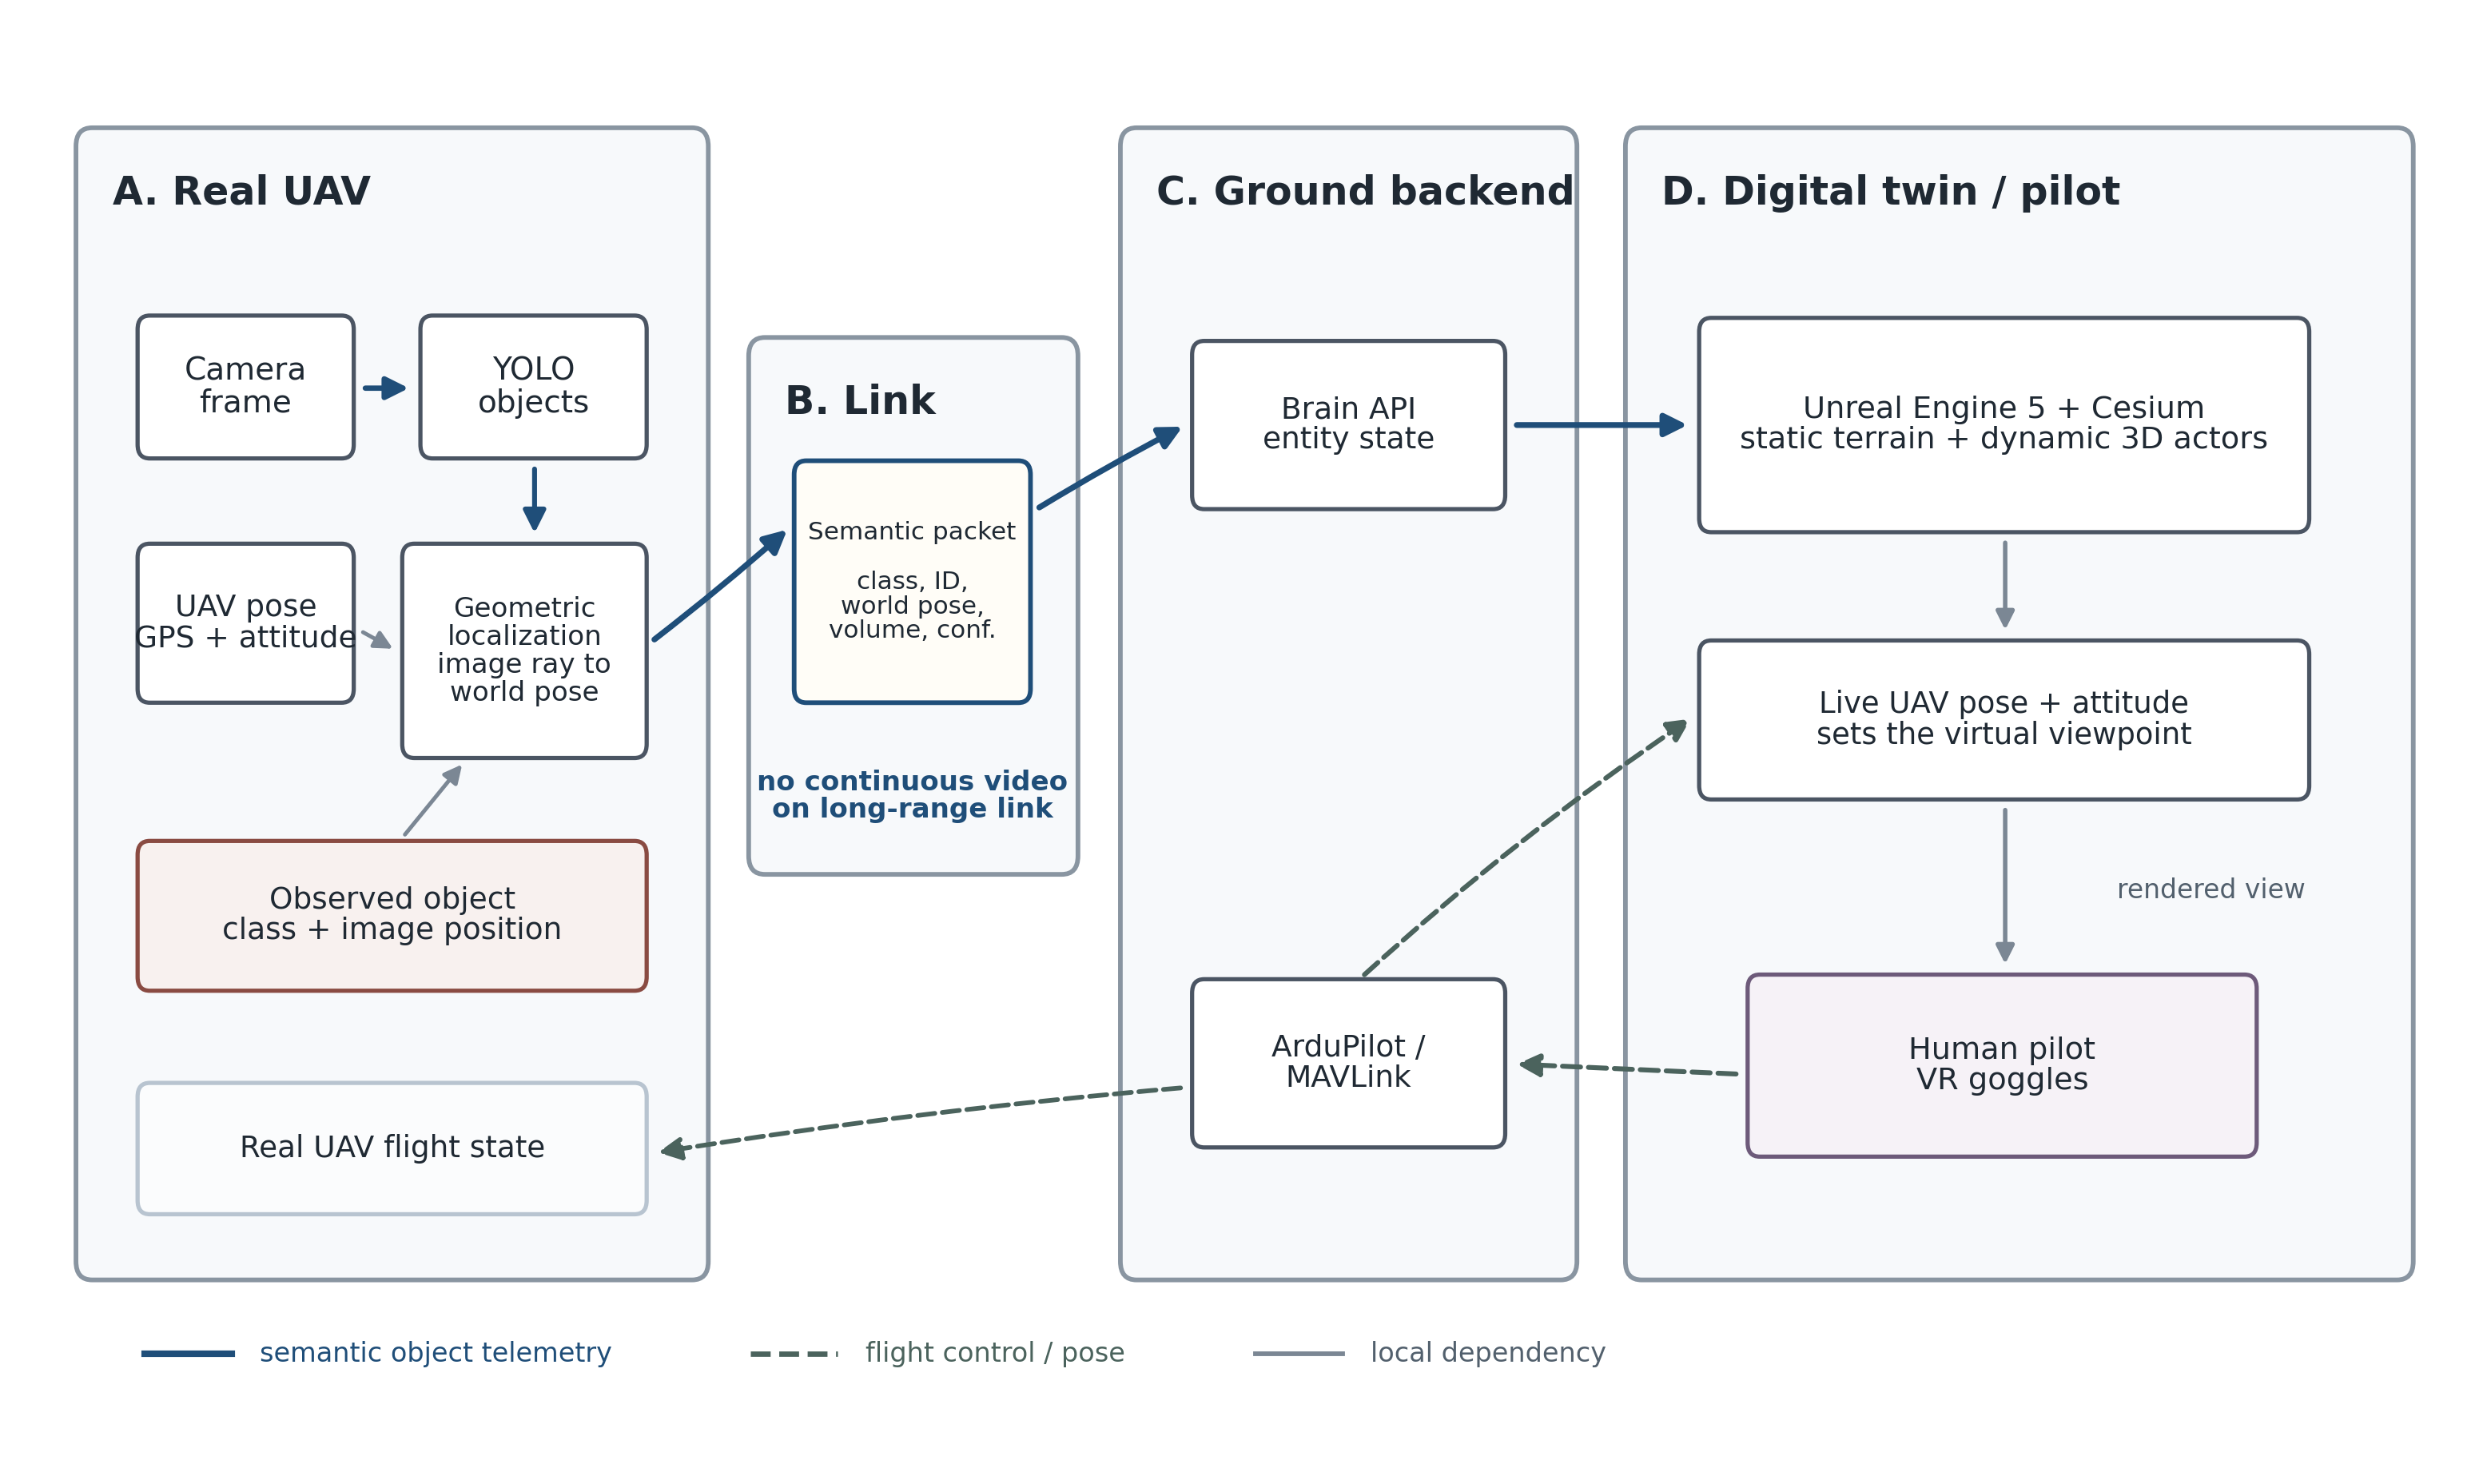
\includegraphics[width=\linewidth]{figures/pipeline_b_architecture.png}
    \caption{Pipeline B runtime flow. The UAV or upstream perception source detects objects with YOLO or another detector, estimates object world coordinates under calibrated camera and pose assumptions, and sends compact semantic telemetry to the ground station. Brain publishes the live entity layer, while Unreal Engine, Cesium terrain, ArduPilot telemetry, and the live object layer are fused into an auxiliary VR operator display. Solid arrows denote semantic object telemetry, dashed arrows denote flight-control and pose feedback, and thin gray arrows denote local dependencies.}
    \label{fig:pipeline-b-architecture}
\end{figure}

\subsection{Runtime Data Flow}

The implemented runtime contract is organized around two HTTP interfaces:

\begin{enumerate}
    \item A detection source publishes objects to \code{POST /api/obstacles}.
    \item Brain normalizes source identity, class, confidence, timestamp, and position.
    \item Brain exposes the current operator-display state through \code{GET /api/ui/data}.
    \item \code{UPorceTelemetryComponent} in Unreal polls the state endpoint.
    \item Unreal spawns, updates, or despawns actors using \code{entity\_id} or \code{object\_id}.
    \item The VR-equipped operator observes the reconstructed entity layer in the digital twin.
\end{enumerate}

\begin{table}[H]
\centering
\caption{Pipeline B runtime data flow.}
\label{tab:pipeline-b-runtime}
\begin{tabular}{@{}lll@{}}
\toprule
Stage & Producer & Consumer \\
\midrule
Object detection & YOLO or detection source & Telemetry encoder \\
Estimated georeferencing & UAV pose + camera assumptions & Detection message \\
Object ingest & Detection sender & Brain endpoint \\
State publication & Brain & Unreal component \\
Actor reconstruction & Unreal component & VR operator display \\
\bottomrule
\end{tabular}
\end{table}

\subsection{Entity Contract}

The essential telemetry fields are:

\begin{itemize}
    \item stable \code{entity\_id} or \code{object\_id};
    \item object class;
    \item confidence score;
    \item \code{lat}/\code{lon} geospatial position when available;
    \item \code{world\_m} local coordinates when available;
    \item approximate footprint, volume, or class-specific geometry;
    \item timestamp, source identifier, and source metadata;
    \item stale-state and uncertainty fields for operator display \tbd{TBD-SAFETY freshness and uncertainty fields}.
\end{itemize}

\subsection{VR Operator Display Requirements}

For VRIH, the display must be specified as an immersive operator interface rather than a generic 3D visualization. A publishable method section must define:

\begin{itemize}
    \item headset or head-mounted display model and runtime \tbd{TBD-DEMO HMD configuration};
    \item viewpoint modes, such as UAV-centric, external chase, top-down inspection, or operator-selected viewpoints \tbd{TBD-DEMO viewpoint modes};
    \item visual encoding of class, confidence, age, and stale state \tbd{TBD-SAFETY display encoding};
    \item interaction model for inspecting entities, filtering classes, and reading uncertainty \tbd{TBD-HUMAN interaction model};
    \item fallback behavior when detections, pose, or network updates are stale \tbd{TBD-SAFETY fallback rule}.
\end{itemize}

\subsection{Georeferencing Assumptions}

The current georeferencing claim must be treated as estimated georeferencing under calibrated camera and pose assumptions, not as a proven localization result. A publishable method section must specify:

\begin{itemize}
    \item camera intrinsics, distortion model, and image resolution \tbd{TBD-GEO camera calibration};
    \item camera-to-body extrinsics and mount roll, pitch, and yaw \tbd{TBD-GEO extrinsic calibration};
    \item UAV pose, attitude, GNSS source, and timestamp synchronization \tbd{TBD-GEO synchronization error};
    \item terrain or ground-plane intersection assumptions \tbd{TBD-GEO terrain model};
    \item propagation of bounding-box, pose, attitude, and map uncertainty into object-position uncertainty \tbd{TBD-SAFETY uncertainty radius};
    \item operating envelope where projection error remains acceptable \tbd{TBD-SAFETY allowed operating envelope}.
\end{itemize}

\section{Current Readiness and Hardware Dependence}

Some parts of the paper can be completed immediately from the existing software, logs, simulator, and controlled replay tools. These software-only tests are preparatory evidence; they are not sufficient on their own for a VRIH research-paper claim about a VR headset operator display. The submission-critical evidence still requires the real UAV or instrumented detection source, calibrated camera assumptions, VR headset, and human operators. Table~\ref{tab:readiness} separates those two categories so that the remaining work is explicit.

\begin{table}[H]
\centering
\small
\caption{Work packages that can be completed now versus work requiring hardware.}
\label{tab:readiness}
\begin{tabular}{@{}L{0.22\linewidth}L{0.30\linewidth}L{0.24\linewidth}L{0.14\linewidth}@{}}
\toprule
Evidence item & Can be completed now & Requires hardware & Status \\
\midrule
VRIH framing & Rewrite title, abstract, introduction, contribution, and conclusion around VR/HMD operator display. & No. & Done in this draft \\
Runtime contract & Document \code{POST /api/obstacles}, \code{GET /api/ui/data}, entity fields, actor lifecycle, and display semantics. & No. & Drafted \\
Bandwidth benchmark & Compute message size, update rate, mean bitrate, p95 bitrate, and packet rate from logs or synthetic/replayed detections. & Real mission logs improve validity but are not strictly required for first benchmark. & \tbd{TBD-BW} \\
Brain-to-Unreal latency & Instrument sender, Brain ingest, state publication, Unreal polling, and actor update on local or lab network. & HMD not needed for this partial latency segment. & \tbd{TBD-LAT partial} \\
Packet loss and jitter & Inject controlled delay, drop, and interruption into semantic telemetry and observe stale-state behavior. & No, unless validating over a real radio link. & \tbd{TBD-LOSS} \\
Synthetic tracking & Replay known trajectories and measure ID switches, stale duration, and fragmentation. & No for synthetic validation; yes for real motion validation. & \tbd{TBD-TRACK synthetic} \\
VR demonstration & Capture screenshots and video of pilot-side VR display running the implemented prototype. & Yes: HMD and running Unreal VR configuration. & \tbd{TBD-DEMO} \\
Drone-to-VR latency & Measure source event to visible headset update. & Yes: real or instrumented detection source plus HMD timing/capture. & \tbd{TBD-LAT e2e} \\
Geospatial error & Compare reconstructed object positions against surveyed or RTK/GNSS ground truth. & Yes: calibrated camera/pose and ground truth objects or controlled flight. & \tbd{TBD-GEO} \\
Human operator utility & Compare video-only, map-only, non-immersive hybrid, and VR digital twin conditions. & Yes: HMD, task scenarios, participants, and protocol approval if needed. & \tbd{TBD-HUMAN} \\
Low-visibility claims & Validate RGB/thermal/LiDAR/radar behavior in night, fog, glare, smoke, or equivalent conditions. & Yes: sensor and environment-specific trials. & \tbd{TBD-LOWVIS} \\
\bottomrule
\end{tabular}
\normalsize
\end{table}

\section{Claim-to-Evidence Map}

\small
\begin{longtable}{@{}L{0.24\linewidth}L{0.34\linewidth}L{0.14\linewidth}L{0.18\linewidth}@{}}
\caption{Claims retained in the paper and evidence required before submission.}
\label{tab:claim-evidence}\\
\toprule
Claim & Required evidence & Status & Acceptance criterion \\
\midrule
\endfirsthead
\toprule
Claim & Required evidence & Status & Acceptance criterion \\
\midrule
\endhead
A real VR digital-twin operator display has been developed. & Screenshots, videos, configuration records, and execution logs showing the UAV-to-Brain-to-Unreal/VR path operating end to end. & \tbd{TBD-DEMO} & Demonstration material shows object ingestion, actor update, and pilot-side VR visualization without relying only on mock diagrams. \\
Semantic telemetry can reduce communication load relative to video. & Bitrate comparison against fixed video baselines with identical mission duration. & \tbd{TBD-BW} & Semantic stream uses substantially less bandwidth while preserving required entity state. \\
Actor updates can be shown with low drone-to-pilot delay. & Synchronized timing from UAV or detector publication to Brain ingest, state publication, Unreal update, and VR-headset-visible actor refresh. & \tbd{TBD-LAT} & P95 latency stays below the operator-display threshold selected in the experiment. \\
Estimated object positions are operationally useful. & Ground-truth comparison over range, altitude, class, and terrain conditions. & \tbd{TBD-GEO} & Error distribution remains inside the declared uncertainty envelope. \\
The display degrades gracefully under packet loss. & Controlled loss, jitter, and interruption experiments against video-only and hybrid baselines. & \tbd{TBD-LOSS} & Stale entities are visible as stale and do not appear as fresh truth. \\
Entity persistence improves operator context. & Tracking metrics, stale-object duration, identity switches, and fragmentation. & \tbd{TBD-TRACK} & Identity stability improves without hiding missed detections. \\
The display helps human operators. & Controlled pilot study with task success, near misses, workload, NASA-TLX, SAGAT, SART, or equivalent awareness measures. & \tbd{TBD-HUMAN} & Operator benefit is statistically or operationally meaningful without increased overtrust. \\
Low-visibility rendering is useful only when sensors still detect hazards. & Sensor-specific trials for RGB, thermal, LiDAR, radar, or other inputs. & \tbd{TBD-LOWVIS} & Display explicitly distinguishes observed, inferred, stale, and missing objects. \\
\bottomrule
\end{longtable}
\normalsize

\section{Evaluation Protocol}

\subsection{Real-System Demonstration Artifacts}

The first submission-critical evidence is not a metric but proof that the implemented prototype actually runs as claimed. The demonstration package should show the runtime chain from detections to Brain state to Unreal actor reconstruction to pilot-side VR display.

\begin{table}[H]
\centering
\small
\caption{Real-system demonstration placeholders.}
\label{tab:demo-placeholder}
\begin{tabular}{@{}L{0.22\linewidth}L{0.30\linewidth}L{0.18\linewidth}L{0.20\linewidth}@{}}
\toprule
Artifact & Purpose & Status & Acceptance criterion \\
\midrule
Screenshots from the VR digital twin & Show the HMD-facing view, terrain context, reconstructed dynamic entities, confidence, and stale-state encoding. & \tbd{TBD-DEMO screenshots} & Captures correspond to the implemented system rather than illustrative mockups. \\
Video of system operation & Show live spawn, update, persistence, and despawn behavior during operation. & \tbd{TBD-DEMO video} & Video includes enough context to connect detections, telemetry, and VR visualization. \\
Runtime logs and configuration & Support reproducibility of the demonstrated setup. & \tbd{TBD-DEMO logs} & Logs identify endpoints, polling rate, timestamps, HMD runtime, headset mode, and display configuration. \\
\bottomrule
\end{tabular}
\normalsize
\end{table}

\subsection{Bandwidth Versus Video}

This experiment can be prepared immediately from synthetic or replayed detection streams. It becomes stronger when repeated with real mission logs and synchronized video baselines.

\begin{table}[H]
\centering
\small
\caption{Bandwidth results placeholder.}
\label{tab:bandwidth-placeholder}
\begin{tabular}{@{}L{0.18\linewidth}L{0.21\linewidth}L{0.20\linewidth}L{0.08\linewidth}L{0.18\linewidth}@{}}
\toprule
Metric & Baseline & Pipeline B & Status & Acceptance criterion \\
\midrule
Mean bitrate & H.264, H.265, WebRTC FPV & \tbd{TBD-BW mean bitrate} & TBD & Lower bitrate for same scenario duration \\
P95 bitrate & Same codec and link profile & \tbd{TBD-BW p95 bitrate} & TBD & Reduced p95 load without entity loss \\
Packet rate & Same mission duration & \tbd{TBD-BW packet rate} & TBD & Compatible with target link budget \\
Entity completeness & Ground-truth or replayed entity stream & \tbd{TBD-BW completeness} & TBD & Bandwidth reduction does not hide required entity state \\
\bottomrule
\end{tabular}
\normalsize
\end{table}

\subsection{End-to-End Latency}

Latency must be decomposed because some segments can be measured now and some require the HMD. Brain ingest, state publication, and Unreal actor update can be instrumented without a real drone. Drone-to-pilot visible latency requires the HMD and a real or instrumented detection source.

\begin{table}[H]
\centering
\small
\caption{Latency results placeholder.}
\label{tab:latency-placeholder}
\begin{tabular}{@{}L{0.18\linewidth}L{0.21\linewidth}L{0.20\linewidth}L{0.08\linewidth}L{0.18\linewidth}@{}}
\toprule
Metric & Baseline & Pipeline B & Status & Acceptance criterion \\
\midrule
Detector publication to Brain ingest & Synchronized detector timestamp and Brain receive log & \tbd{TBD-LAT detector-to-brain} & TBD & Below selected runtime threshold \\
Brain to Unreal actor update & Polling and render logs & \tbd{TBD-LAT actor update} & TBD & P95 below operator-display threshold \\
Unreal update to VR headset display & Unreal timing, headset capture, or instrumented presentation timestamp & \tbd{TBD-LAT vr-display} & TBD & Visible update remains within the declared pilot-display threshold \\
End-to-end source-to-HMD visible update & Detector event to actor visible to the VR-equipped pilot & \tbd{TBD-LAT e2e-source-to-vr} & TBD & No unnoticed stale display \\
\bottomrule
\end{tabular}
\normalsize
\end{table}

\subsection{Geospatial Error}

This validation is hardware-dependent if the paper claims real-world positioning accuracy. Synthetic coordinates or manually injected positions can test software consistency, but not camera-to-world georeferencing.

\begin{table}[H]
\centering
\small
\caption{Geospatial error results placeholder.}
\label{tab:geo-placeholder}
\begin{tabular}{@{}L{0.18\linewidth}L{0.21\linewidth}L{0.20\linewidth}L{0.08\linewidth}L{0.18\linewidth}@{}}
\toprule
Metric & Baseline & Pipeline B & Status & Acceptance criterion \\
\midrule
2D position error & RTK/GNSS or surveyed ground truth & \tbd{TBD-GEO 2D error} & TBD & Error inside declared uncertainty radius \\
3D position error & Ground-truth height or volume & \tbd{TBD-GEO 3D error} & TBD & Height error acceptable for visualization \\
Error by range & Near, mid, far detections & \tbd{TBD-GEO by range} & TBD & Error envelope reported by range bin \\
Uncertainty calibration & Measured error versus displayed uncertainty & \tbd{TBD-GEO uncertainty calibration} & TBD & Displayed uncertainty is not overconfident \\
\bottomrule
\end{tabular}
\normalsize
\end{table}

\subsection{Packet Loss and Jitter Robustness}

This experiment can be implemented now with a network impairment layer or replay tool. It should test the semantic display against video-only and hybrid baselines, with special attention to stale-state visualization.

\begin{table}[H]
\centering
\small
\caption{Packet-loss and jitter results placeholder.}
\label{tab:loss-placeholder}
\begin{tabular}{@{}L{0.18\linewidth}L{0.21\linewidth}L{0.20\linewidth}L{0.08\linewidth}L{0.18\linewidth}@{}}
\toprule
Metric & Baseline & Pipeline B & Status & Acceptance criterion \\
\midrule
Packet loss degradation & Video-only and hybrid display & \tbd{TBD-LOSS loss sweep} & TBD & Graceful stale-state behavior \\
Jitter sensitivity & Fixed jitter profiles & \tbd{TBD-LOSS jitter sweep} & TBD & No false freshness under delayed updates \\
Interruption recovery & Link interruption scenario & \tbd{TBD-LOSS recovery} & TBD & Recovery state visible to operator \\
False freshness rate & Delayed or dropped updates & \tbd{TBD-LOSS false freshness} & TBD & Stale data is not presented as fresh state \\
\bottomrule
\end{tabular}
\normalsize
\end{table}

\subsection{Dynamic Object Tracking}

Tracking can first be evaluated with replayed or synthetic trajectories. A stronger validation requires real moving objects, synchronized ground truth, and class-specific occlusion or detection-loss scenarios.

\begin{table}[H]
\centering
\small
\caption{Tracking results placeholder.}
\label{tab:track-placeholder}
\begin{tabular}{@{}L{0.18\linewidth}L{0.21\linewidth}L{0.20\linewidth}L{0.08\linewidth}L{0.18\linewidth}@{}}
\toprule
Metric & Baseline & Pipeline B & Status & Acceptance criterion \\
\midrule
ID switches & Ground-truth trajectories & \tbd{TBD-TRACK ID switches} & TBD & ID switches reported and bounded \\
Track fragmentation & Moving-object trial & \tbd{TBD-TRACK fragmentation} & TBD & Fragmentation does not hide uncertainty \\
Stale-object duration & Controlled occlusion/loss & \tbd{TBD-TRACK stale duration} & TBD & Stale state visibly encoded \\
Despawn correctness & Known disappearance events & \tbd{TBD-TRACK despawn} & TBD & Actors are removed or marked stale according to declared policy \\
\bottomrule
\end{tabular}
\normalsize
\end{table}

\subsection{Human Operator Utility}

For a VR-focused journal, the human-operator evaluation is not decorative. It is the evidence that the immersive display changes the operator task. A minimum study should compare video-only, map-only, non-immersive hybrid, and VR digital-twin conditions on the same mission scenarios.

\begin{table}[H]
\centering
\small
\caption{Human-operator study placeholder.}
\label{tab:human-placeholder}
\begin{tabular}{@{}L{0.18\linewidth}L{0.21\linewidth}L{0.20\linewidth}L{0.08\linewidth}L{0.18\linewidth}@{}}
\toprule
Metric & Baseline & Pipeline B & Status & Acceptance criterion \\
\midrule
Task success & Video-only, map-only, hybrid & \tbd{TBD-HUMAN task success} & TBD & Improvement or non-inferiority with lower link load \\
Spatial awareness & SAGAT, SART, or equivalent & \tbd{TBD-HUMAN awareness} & TBD & Operators better identify object position, age, and relevance \\
Workload & NASA-TLX or equivalent & \tbd{TBD-HUMAN workload} & TBD & Benefit without unacceptable cognitive load \\
Near misses or unsafe decisions & Same operator tasks & \tbd{TBD-HUMAN near misses} & TBD & No increase in safety-relevant events \\
Overtrust & Post-task questionnaire and stale-state trials & \tbd{TBD-HUMAN overtrust} & TBD & Operators notice uncertainty and stale objects \\
\bottomrule
\end{tabular}
\normalsize
\end{table}

\subsection{Low-Visibility and Sensor Dependence}

Low-visibility claims must remain out of the main contribution unless sensor-specific evidence is collected. The current paper can define the protocol now, but the claim requires hardware and environmental trials.

\begin{table}[H]
\centering
\small
\caption{Low-visibility validation placeholder.}
\label{tab:lowvis-placeholder}
\begin{tabular}{@{}L{0.18\linewidth}L{0.21\linewidth}L{0.20\linewidth}L{0.08\linewidth}L{0.18\linewidth}@{}}
\toprule
Metric & Baseline & Pipeline B & Status & Acceptance criterion \\
\midrule
RGB night or glare & Raw video and semantic display & \tbd{TBD-LOWVIS RGB} & TBD & Missed detections explicitly represented \\
Sensor fallback & Thermal, LiDAR, radar, or equivalent & \tbd{TBD-LOWVIS sensor fallback} & TBD & Sensor limits reported by condition \\
Uncertainty display & Display variants & \tbd{TBD-LOWVIS uncertainty} & TBD & Operator can identify missing or stale state \\
\bottomrule
\end{tabular}
\normalsize
\end{table}

\section{Limitations and Safety Envelope}

Pipeline B can mislead an operator if its uncertainty is hidden. The following limitations are part of the current system definition:

\begin{itemize}
    \item False negatives are safety-critical because absent objects may simply be undetected.
    \item Stale actors can look authoritative unless age and confidence are visualized.
    \item A visually stable synthetic scene can increase overtrust.
    \item Object metadata, timestamps, and geolocation can still be privacy-sensitive.
    \item Night, smoke, fog, haze, glare, and occlusion reduce sensor performance unless alternative sensors are validated.
    \item Cesium, map, terrain, and home-origin errors can become actor-placement errors.
    \item BVLOS use requires detect-and-avoid, command-and-control reliability, operational-design-domain limits, and regulatory compliance beyond this display.
    \item VR can introduce simulator sickness, attentional tunneling, fatigue, and display occlusion that must be considered in the human study.
\end{itemize}

Before any safety-relevant claim, the following thresholds must be defined and measured:

\begin{itemize}
    \item maximum stale-object age \tbd{TBD-SAFETY max stale age};
    \item maximum position uncertainty radius \tbd{TBD-SAFETY max uncertainty radius};
    \item minimum detection confidence for confirmed actor display \tbd{TBD-SAFETY minimum confidence};
    \item fallback rule when telemetry, detections, or pose become stale \tbd{TBD-SAFETY fallback rule};
    \item allowed operating envelope by altitude, range, speed, terrain, lighting, and sensor configuration \tbd{TBD-SAFETY allowed operating envelope}.
\end{itemize}

\section{VRIH Submission Package Still Required}

Before submission, the working draft must be converted to the VRIH author template and accompanied by the journal's required submission materials. The following items can be prepared now:

\begin{itemize}
    \item title page with all author affiliations and corresponding author details \tbd{author affiliations and corresponding author};
    \item abstract under 250 words, already satisfied in this draft;
    \item one to seven keywords, already satisfied in this draft;
    \item highlights file with three to five concise bullet points \tbd{VRIH highlights file};
    \item graphical abstract or representative visual, if used \tbd{VR digital-twin screenshot};
    \item author contribution statement using CRediT roles \tbd{CRediT roles};
    \item conflict-of-interest statement \tbd{declarations};
    \item data and code availability statement \tbd{data/code availability};
    \item ethics statement if human-operator tests are performed \tbd{human-study ethics requirement}.
\end{itemize}

\section{Conclusion}

Pipeline B is best framed for VRIH as a human-in-the-loop VR digital-twin operator display for dynamic UAV scene reconstruction from in-flight detections. Its current contribution is the implemented integration path from detection messages through Brain state publication into Unreal/Cesium actor reconstruction, together with a concrete validation protocol for measuring whether the approach improves operator awareness under degraded communication conditions.

The manuscript is not yet a completed experimental paper. The work that can be completed immediately is now explicit: VRIH-aligned framing, runtime contract, instrumentation plan, bandwidth benchmark design, partial latency instrumentation, packet-loss testing, and synthetic tracking evaluation. The remaining publication-critical evidence requires hardware: HMD demonstration, source-to-headset latency, calibrated geospatial error, human-operator study, and any low-visibility sensor claims.

\begin{thebibliography}{9}

\bibitem{shao2022task}
J. Shao, X. Zhang, and J. Zhang, ``Task-Oriented Communication for Edge Video Analytics,'' arXiv:2211.14049, 2022. \url{https://arxiv.org/abs/2211.14049}

\bibitem{nasa2005smartcam}
NASA NTRS, ``A Hybrid Synthetic Vision System for the Tele-operation of Unmanned Vehicles,'' 2005. \url{https://ntrs.nasa.gov/citations/20050217300}

\bibitem{sehad2023digitaltwin}
N. Sehad et al., ``Towards Enabling Reliable Immersive Teleoperation Through Digital Twin: A UAV Command and Control Use Case,'' arXiv:2308.14524, 2023. \url{https://arxiv.org/abs/2308.14524}

\bibitem{shah2017airsim}
S. Shah, D. Dey, C. Lovett, and A. Kapoor, ``AirSim: High-Fidelity Visual and Physical Simulation for Autonomous Vehicles,'' arXiv:1705.05065, 2017. \url{https://arxiv.org/abs/1705.05065}

\bibitem{cao2023uavdetection}
Z. Cao, L. Kooistra, W. Wang, L. Guo, and J. Valente, ``Real-Time Object Detection Based on UAV Remote Sensing: A Systematic Literature Review,'' \emph{Drones}, vol. 7, no. 10, 620, 2023. \url{https://www.mdpi.com/2504-446X/7/10/620}

\bibitem{barber2006geolocation}
D. B. Barber, J. D. Redding, T. W. McLain, R. W. Beard, and C. N. Taylor, ``Vision-based Target Geo-location Using a Fixed-wing Miniature Air Vehicle,'' \emph{Journal of Intelligent and Robotic Systems}, 2006. \url{https://scholarsarchive.byu.edu/facpub/1502/}

\bibitem{isprs2016geolocation}
ISPRS Archives, ``Precise Target Geolocation and Tracking Based on UAV Video Imagery,'' 2016. \url{https://isprs-archives.copernicus.org/articles/XLI-B6/243/2016/}

\bibitem{faa2025bvlos}
Federal Register, ``Normalizing Unmanned Aircraft Systems Beyond Visual Line of Sight Operations,'' 2025. \url{https://www.federalregister.gov/documents/2025/08/07/2025-14992/normalizing-unmanned-aircraft-systems-beyond-visual-line-of-sight-operations}

\end{thebibliography}

\end{document}
